\section{Integración de Mezfer Insider con Control Manager Siso}
Control Manager Siso (CMS) es el sistema de inicio de sesión de Siso ERP, un sistema ERP que permite realizar la gestión de distintos aspectos de una empresa. Cuando un cliente compra una licencia de Siso ERP, se le otorgan un correo y contraseña que podrán usar para iniciar sesión mediante CMS y acceder a sus empresas.

Quienes son administradores de CMS tienen acceso al panel de administración, donde se les permite gestionar a los usuarios y empresas del sistema Siso ERP.

Para poder crear empresas (que son tratadas como aplicaciones web), CMS realiza peticiones a diferentes endpoints de la API de la nueva empresa y, dependiendo de la respuesta que se reciba, se registrará correctamente a la base de datos o no. Lo mismo aplica para cuando se quiere asignar un usuario a una empresa y cuando se quiere ingresar a la empresa.
    \subsection{Creación de endpoints en la API de Mezfer Insider}
En la API de Mezfer Insider deben existir tres endpoints que permitirán a CMS realizar las acciones necesarias para registrar el proyecto en su base de datos.

El primer endpoint consiste en que se procese la información de la empresa. Mediante el Frontend, el administrador ingresa la información de la empresa en el formulario correspondiente y esta es enviada a la API; dependiendo de las necesidades del proyecto, esta información puede ser procesada o solamente recibida. En el caso de Mezfer Insider, esta información no requiere ser almacenada ni requiere ser procesada. Se debe retornar una respuesta con el código de estado de respuesta HTTP 202, indicando así que la petición se ha recibido, pero no se ha actuado.

El segundo endpoint consiste en vincular a un usuario con la empresa para indicar al sistema que ese usuario va a poder acceder a la empresa. En CMS, el administrador se encargará de asignarle la empresa al usuario, lo que enviará una nueva petición a la API para permitir la vinculación. La API recibirá el usuario y la empresa que están siendo vinuclados, esta información será procesada de acuerdo a las necesidades del proyecto. La API enviará un código de estado de respuesta HTTP 200, indicando que la operación ha sido realizada con éxito.

El tercer endpoint permitirá al usuario acceder a la empresa. Este endpoint es un poco más complejo, pues requiere el procesamiento de tokens JWT. Cuando el usuario ingresa en la empresa, CMS envía en la URL un token JWT con cierta información del usuario.
Para Mezfer Insider, esta información es importante pues se considera que todos los usuarios que ingresen mediante CMS son administradores, así que debe de quedar registro de ellos. Cuando se recupera el token de la URL, este es decodificado y se lee cierta información que posteriormente es utilizada para realizar otra petición a la API de CMS y así obtener la información completa del usuario; con esto se crea un objeto con la información que se requiere del usuario para guardarla en la base de datos. Una vez guardado el usuario, se procede a crear un token JWT propio de Mezfer Insider que posteriormente será almacenado en una cookie, de esta manera se creará una cookie de sesión que será de utilidad para permitir al usuario realizar distintas acciones dentro de la aplicación. Este proceso se repite cada que un usuario ingresa a la empresa, por lo que debe validarse la existencia del usuario en la base de datos para evitar que se intente guardar nuevamente.
    \subsection{Creación de la empresa, vinculación del usuario e ingreso}
Con los endpoints creados, ya es posible realizar todas las acciones necesarias para integrar Mezfer Insider con CMS.

Lo primero que se tiene que hacer es crear la empresa, y para eso se llena un formulario con todos los datos de la empresa.
    \begin{figure}[H]
        \begin{center}
            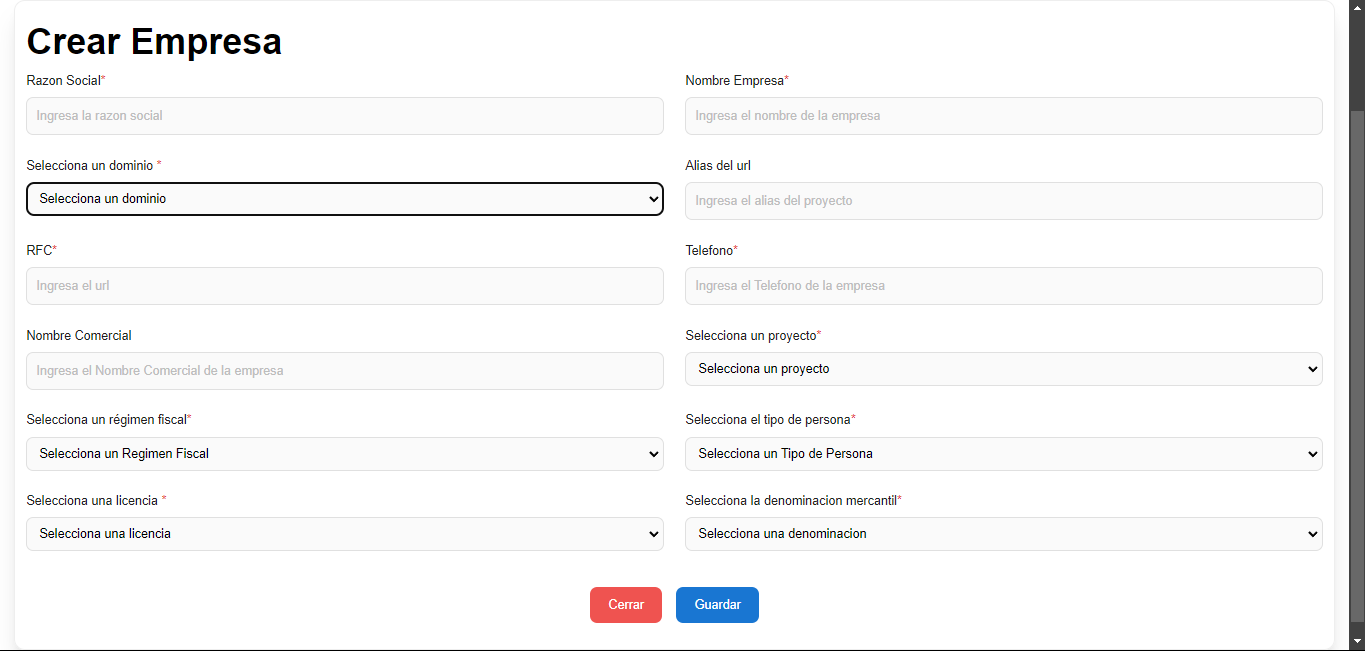
\includegraphics[scale=0.4]{img/actividades/integracion/formulario-empresa.png}
            \caption{Formulario para la creación de empresa.}
            \label{fig:formulario-empresa}
        \end{center}
    \end{figure}
Posteriormente, el usuario debe ser vinculado con la empresa.
    \begin{figure}[H]
        \begin{center}
            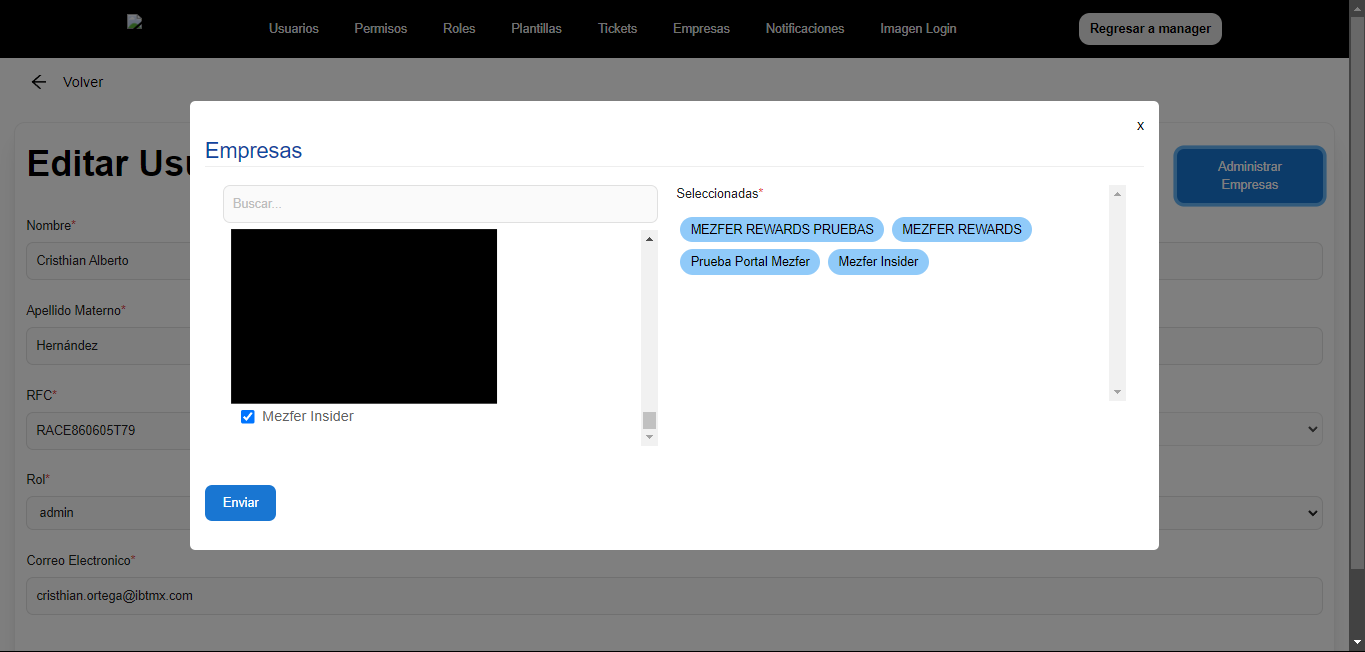
\includegraphics[scale=0.4]{img/actividades/integracion/vincular-usuario.png}
            \caption{Vinculación de usuario con empresa.}
            \label{fig:vincular-usuario}
        \end{center}
    \end{figure}
Y con esto realizado, el usuario ya podrá tener acceso a la empresa.
    \begin{figure}[H]
        \begin{center}
            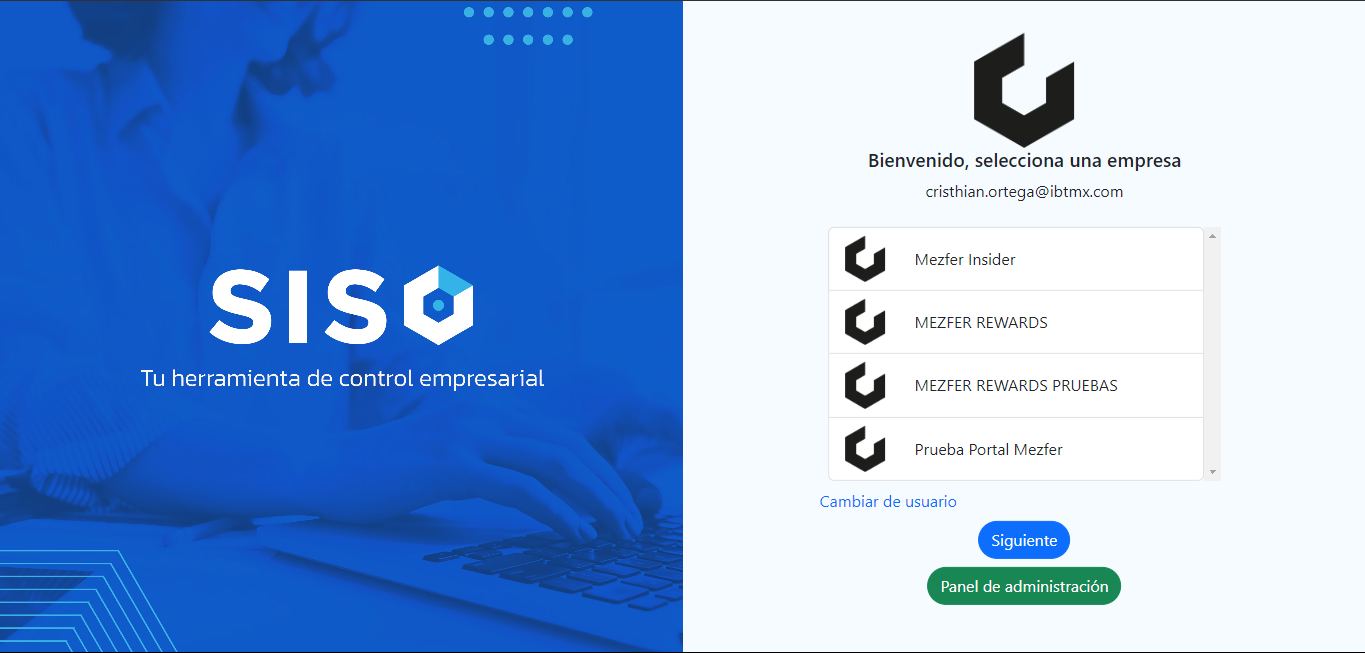
\includegraphics[scale=0.4]{img/actividades/integracion/ingreso-empresa.png}
            \caption{Selección de empresa.}
            \label{fig:ingreso-empresa}
        \end{center}
    \end{figure}